%%%% Semesterprojekt rapport gruppe 2 %%%%
%%%% Elektronik Q1/Q2 2016 %%%%

% Kan anvendes til journaler eller afleveringer
\documentclass[11pt, a4paper, twoside, openany]{memoir}

\usepackage[utf8]{inputenc}		% Dansk input encoding (tegn)
\usepackage[english, danish]{babel}		% Danske formuleringer / orddeling
\usepackage[T1]{fontenc}		% Output-indkodning af tegnsaet (T1)


%%% Memoir indstillinger
%% Afstand mellem afsnit og videre
%% NIX PILLE - medmindre strengt nødvendigt
\setaftersubsubsecskip{6pt}	
\setbeforesubsubsecskip{ 6pt}
%\setaftersubsecskip{6pt}
%\setbeforesubsecskip{-\baselineskip}
%\setaftersecskip{6pt}
%\setbeforesecskip{-\baselineskip}
%\setaftersecskip{1ex}


\raggedbottom



\chapterstyle{section}

% ¤¤ Marginer ¤¤ %
\setlrmarginsandblock{3.5cm}{2.5cm}{*}		% \setlrmarginsandblock{Indbinding}{Kant}{Ratio}
\setulmarginsandblock{3.0cm}{2.5cm}{*}		% \setulmarginsandblock{Top}{Bund}{Ratio}
\checkandfixthelayout

%%% Font valg %%%
\usepackage{mathpazo}	%Palatinofont - matematikformler
\usepackage{eulervm}		%Palatinofont

%%% FIGURER OG TABELLER %%%
\usepackage{graphicx} 						% Haandtering af eksterne billeder (JPG, PNG, PDF)

\usepackage[export]{adjustbox}

\usepackage{subfig}

\usepackage{multirow}                		% Fletning af raekker og kolonner (\multicolumn og \multirow)
\usepackage{colortbl} 						% Farver i tabeller (fx \columncolor, \rowcolor og \cellcolor)
\usepackage[dvipsnames]{xcolor}				% Definer farver med \definecolor. Se mere: http://en.wikibooks.org/wiki/LaTeX/Colors
%\usepackage{flafter}						% Soerger for at floats ikke optraeder i teksten foer deres erence
\usepackage{float}							% Muliggoer eksakt placering af floats, f.eks. \begin{figure}[H]
\usepackage{multicol}         	        	% Muliggoer tekst i spalter
%\usepackage{rotating}						% Rotation af tekst med \begin{sideways}...\end{sideways}
\usepackage{booktabs}
\usepackage{bigstrut}	% Excel2latex måskeh
\usepackage{tabularx}

%%% ¤¤ Matematik mm. %%%
\usepackage{amsmath,amssymb,stmaryrd} 		% Avancerede matematik-udvidelser
\usepackage{mathtools}						% Andre matematik- og tegnudvidelser
\usepackage{textcomp}                 		% Symbol-udvidelser (f.eks. promille-tegn med \textperthousand )
\usepackage{siunitx}						% Flot og konsistent praesentation af tal og enheder med \si{enhed} og \SI{tal}{enhed}
\sisetup{output-decimal-marker = {,}}		% Opsaetning af \SI (DE for komma som decimalseparator) 
\sisetup{exponent-product=\cdot, output-product=\cdot}	%Eksponent er gange tegn, output produkt er gange tegn
\sisetup{digitsep = none}					%Almindeligt komma - ingen mellemrum aka. til eurokomma




%%% MISC %%%
\usepackage{listings}						% Placer kildekode i dokumentet med \begin{lstlisting}...\end{lstlisting}
\definecolor{bg}{HTML}{F0F0F0}
\lstset{language=C++,
				showstringspaces = false,
				backgroundcolor = \color{bg},
                basicstyle=\ttfamily,
                keywordstyle=\color{blue}\ttfamily,
                stringstyle=\color{red}\ttfamily,
                commentstyle=\color{green}\ttfamily,
                morecomment=[l][\color{magenta}]{\#},
                extendedchars=true,
                numbers=left, numberstyle=\tiny,		% Linjenumre
                columns=flexible,						% Kolonnejustering
                breaklines, breakatwhitespace=true,		% Bryd lange linjer
                literate=%
                {æ}{{\ae}}1
                {å}{{\aa}}1
                {ø}{{\o}}1
                {Æ}{{\AE}}1
                {Å}{{\AA}}1
                {Ø}{{\O}}1
}


\usepackage{lipsum}							% Dummy text \lipsum[..]
\usepackage[shortlabels]{enumitem}			% Muliggoer enkelt konfiguration af lister
\usepackage{pdfpages}						% Goer det muligt at inkludere pdf-dokumenter med kommandoen \includepdf[pages={x-y}]{fil.pdf}	
\pdfoptionpdfminorversion=6					% Muliggoer inkludering af pdf dokumenter, af version 1.6 og hoejere

%	¤¤ Afsnitsformatering ¤¤ %
%\setlength{\parindent}{0mm}           		% Stoerrelse af indryk
\setlength{\parskip}{1.5mm}          		% Afstand mellem afsnit ved brug af double Enter
\linespread{1,1}							% Linie afstand

\usepackage{tikz}


% ¤¤ Visuelle  ¤¤ %
\usepackage[colorlinks]{hyperref}			% Danner klikbare referencer (hyperlinks) i dokumentet.
\hypersetup{colorlinks = true,				% Opsaetning af farvede hyperlinks (interne links, citeringer og URL)
	linkcolor = black,
	citecolor = black,
	urlcolor = black
}
\usepackage{url}

%%% REFERENCER %%%
%\usepackage{xr}
%\externaldocument{../dokumentation/dokumentation.tex}



%%% Referencer / Bibliografi %%%
\usepackage[backend=bibtex, sorting=none, style=numeric]{biblatex}
\bibliography{../referencer.bib}






\usepackage[draft, danish]{fixme}
\fxsetup{layout=footnote}

\graphicspath{{../fig/}{../fig}{fig/}{./}}

\usepackage{titlesec}

\setcounter{secnumdepth}{4}

\titleformat{\paragraph}
{\normalfont\normalsize\bfseries}{\theparagraph}{1em}{}
\titlespacing*{\paragraph}
{0pt}{3.25ex plus 1ex minus .2ex}{1.5ex plus .2ex}


%%%% Opsætning af dokument %%%%
\newcommand{\forfatter}{Gruppe 2}
\newcommand{\fag}{INDSÆT KURSUS HER}
\newcommand{\titel}{Semesterprojekt 4 Rapport}
\date{}

\author{\forfatter}
\title{\titel}


\setlength{\beforechapskip}{10pt}
\setlength{\afterchapskip}{10pt}
\begin{document}
%\maketitle
\begin{titlingpage}
%\thispagestyle{title}
\selectlanguage{danish}
		
		\begin{center}
				{\huge\bfseries Projekt Universal Actuator Drive}\\
				\vspace{10pt}
				
				{\Huge\bfseries Rapport}\\
				
				\vspace{20pt}
				
				{Diplomingeniør Elektronik}\\
				{\large Bachelorprojekt Efterår 2017}\\
				
				\vspace{10pt}
				
				Ingeniørhøjskolen Aarhus Universitet\\
				Vejleder: Arne Justesen
				\vspace{10pt}
				
				20. december 2017
				\vspace{10pt}
				\begin{figure}[H]
					\centering
					%\includegraphics[max width=0.9\linewidth]{forside.png}
				\end{figure}
				\vspace{50pt}
				\begin{minipage}{0.25\linewidth}
					\centering
					\hrule
					\vspace{12pt}
					Nicolai H. Fransen\\
					Studienr. 201404672
				\end{minipage}
				\hspace{10pt}
				\begin{minipage}{0.25\linewidth}
					\centering
					\hrule
					\vspace{12pt}
					Jesper Kloster\\
					Studienr. 
				\end{minipage}
				\hspace{10pt}


		\end{center}

\end{titlingpage}
		
		\selectlanguage{danish}
		\begin{abstract}
			
		\end{abstract}
		
		\selectlanguage{english} 
		\begin{abstract}
			
		\end{abstract}
		
		\selectlanguage{danish}
		
		\clearpage
		
	%\setcounter{tocdepth}{2}
	\tableofcontents
	\clearpage
	
	%% Synopsis:
	
	% Indholdsfortegnelse
	% Ansvarsområder
	% Abstract
	
	% Forord
	% Indledning
	% Opgaveformulering
	% Systembeskrivelse
	% Krav(specifikation)
	% Projektbeskrivelse
	%% Projektgennemførsel
	%% Udviklingsprocesser / Arbejdsmetoder
	%% (Udviklingsværktøjer); nødvendigt?
	%% Specifikation og Analyse
	%% Systembetragtning
	%% Systemarkitektur
	
	% Hardware - design og implementering
	%% Design
	%% (De forskellige moduler)
	
	% Software - design og implementering
	
	% Resultater og diskussion
	% Fremtidigt arbejde (?)
	% Konklusion
	% Ordliste (?)
	% Referencer
	
	%\include{<sti/filnavn>}
	\chapter{Kravspecifikation}

%\subsection{Prioritering / Afgrænsning} måske?
%Moscow
Kravene til produktet er prioriteret ved brug af MoSCoW metoden. Her er kravene for produktet inddelt i fire kategorier, hvor de vigtigste elementer er prioriteret højest. \textbf{Must} benævner de krav som er vigtigst at opfylde, og som er absolut nødvendigt for produktet. \textbf{Should} er de krav produktet bør opfylde. \textbf{Could} er kravene som produktet evt. kunne opfylde, hvis projektets tidsramme tillader det. \textbf{Won't} er krav som ikke vil blive opfyldt inden for projektets tidsrammer, men evt. kan tages med i senere iterationer.

\noindent Følgende opdeling viser kravene udvalgt for dette projekt:
\begin{itemize}
	\item[\textbf{Must}]
		\begin{itemize}
			\item Holde konstant udgangsstrøm og -spænding
			\item Have stabil regulering
			\item Ikke påvirke andre moduler ved fejl
			\item Konstrueres med EEE komponenter

		\end{itemize}
	\item[\textbf{Should}]
		\begin{itemize}
			\item Have programmerbar udgangsstrøm og -spænding

		\end{itemize}
	\item[\textbf{Could}] 
		\begin{itemize}
			\item Have overstrømsbeskyttelse på udgangen

		\end{itemize}
	\item[\textbf{Won't}]
		\begin{itemize}
			\item Indeholde galvanisk adskillelse
		\end{itemize}
\end{itemize}
% De krav der er kritisk for selve funktionen af bilen, dvs. bevægelse / styring, er prioriteret højest. Herefter er krav, som afhænger af bla bla bla. Måske.

\begin{figure}[H]
	\centering
	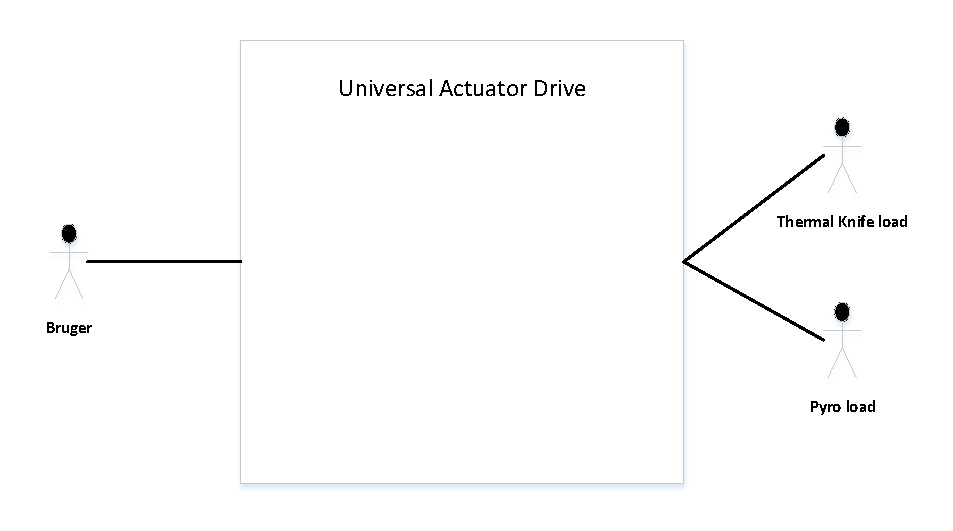
\includegraphics{tex/Kravspecifikation/billeder/AktorkontekstdiagramV1.pdf}
	\caption{Aktør-kontekst diagram}
\end{figure}

\begin{figure}[H]
	\centering
	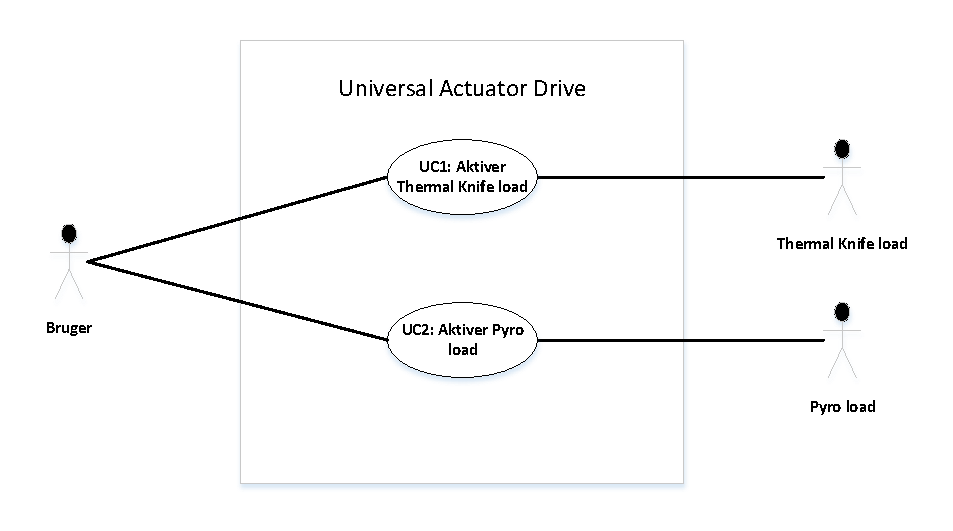
\includegraphics{tex/Kravspecifikation/billeder/UseCasediagramV1.pdf}
	\caption{Use case diagram}
\end{figure}

\section{Aktørbeskrivelse}
I det følgende afsnit beskrives systemets aktører. Ved hver aktør angives typen, samt en kort beskrivelse af aktørens funktion og/eller hvordan de påvirker systemet.

\begin{framed}
	\subsection{Aktør: Bruger}
	\subsubsection*{Type:}
		Primær
	
	\subsubsection*{Beskrivelse:}
		Brugeren interagerer med systemet, ved at indstille den ønskede load type.
\end{framed}

\begin{framed}
	\subsection{Aktør: Thermal Knife load}
	\subsubsection*{Type:}
	Sekundær
	
	\subsubsection*{Beskrivelse:}
	Thermal Knife load er en load type
\end{framed}

\begin{framed}
	\subsection{Aktør: Pyro load}
	\subsubsection*{Type:}
	Sekundær
	
	\subsubsection*{Beskrivelse:}
	Pyro load er en load type
\end{framed}

\clearpage


\section{Fully dressed use cases}

\begin{framed}
	\subsection{Use case 1 - Start bil}
	\subsubsection*{Mål:}
		Initiere bilen så den er klar til kørsel og er klar til at modtage input
		
	\subsubsection*{Initiering:}
		Brugeren
	
	\subsubsection*{Aktører:}
		Brugeren (primær)
	
	\subsubsection*{Referencer:}
		Ingen
	
	\subsubsection*{Samtidige forekomster:}
		En
	
	\subsubsection*{Forudsætning:}
		Bilen er slukket og der er forbindelse fra interface til bil
	
	\subsubsection*{Resultat:}
		Bilens sensorer er tændt, motorer er klar, bilen holder stille
	
	\subsubsection*{Hovedscenarie:}
		\begin{enumerate}
			\item Brugeren vælger via interface ''Start bil''
			\item Bilen monitorerer sensorinputs og rapporterer status 
			\item Bilen udfører motortjek ved at køre bilen lidt frem og derefter tilbage
			\item Bilen rapporterer status
			\item Bilen tænder for- og baglys, blinker med blinklys hvis status er OK 
			\begin{description}
					\item[Extension 1:] Status ikke OK
			\end{description}
			\item Bilen afventer brugerinput
		\end{enumerate}
	
	\subsubsection*{Extensions:}
	\textbf{Extension 1:} Status ikke OK	% Fix layout
		\begin{enumerate}
			\item Bilen rapporterer fejl og forsøger at angive hvilken sensor og/eller motor der fejler
		\end{enumerate}
	
\end{framed}
	

% Skabelon
%\begin{framed}
%\subsubsection{Mål:}
%
%\subsubsection{Initiering:}
%
%\subsubsection{Aktører:}
%
%\subsubsection{Referencer:}
%
%\subsubsection{Samtidige forekomster:}
%
%\subsubsection{Forudsætning:}
%
%\subsubsection{Resultat:}
%
%\subsubsection{Hovedscenarie:}
%
%\subsubsection{Extension:}

\section{Ikke-funktionelle krav}
I dette afsnit beskrives de ikke-funktionelle krav. Her opstilles f.eks. krav om præcision, brugervenlighed samt produktets dimensioner.
\begin{itemize}
			\item Inputspændingen skal være mellem 26-100V
			\item Der må maksimalt trækkes en peak-strøm fra inputkilden på 150\% af inputstrømmen
			\item Skal opretholde en outputspænding på op til 21V ved 2,5A
			\item Der må maksimalt være en ripple-spænding på 50mV pk-pk ved fundamental ripple frekvens
			\item Der må maksimalt være switching spikes på 100mV pk-pk
			\item Skal kunne omsætte op til 75W
			\item Skal operere med et tab på maksimalt 5W %%FIXME
			\item Skal implementeres i et volumen mindre end 17x75x100mm på forsiden af PCB, samt 3x75x100mm på bagsiden PCB'et
			\item Skal kunne operere med en omgivelsestemperatur mellem -35\degreeCelsius  og 65\degreeCelsius
			\item Skal have stabil regulering med 10dB gain og 50 graders fasemargin ved:
				\begin{description}
					\item 21V/2A ved høj og lav indgangsspænding
					\item 5A/2\ohm ved høj og lav indgangsspænding
				\end{description}
			\item Reguleringen skal have en risetime på maksimalt 0,5ms uden overshoot
					
\end{itemize}

	
	
	%\printbibliography[title={Litteraturliste}]

\end{document}